
\begin{figure}[ht]
	\begin{center}
		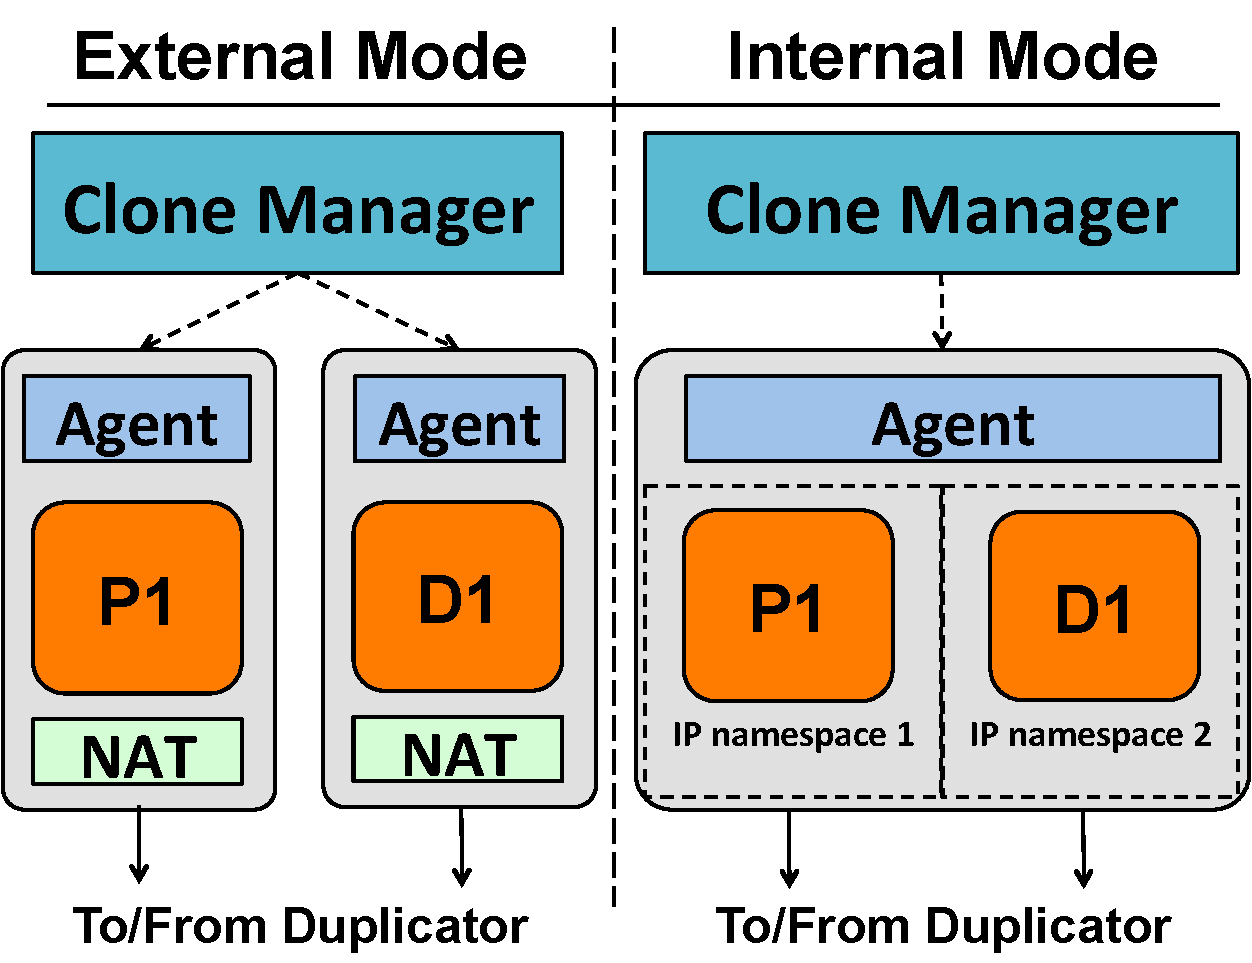
\includegraphics[width=0.9\textwidth]{parikshan/figs/ModesCloning.pdf}
		\caption{External and Internal Mode for live cloning: P1 is the production, and D1 is the debug container, the clone manager interacts with an agent which has drivers to implement live cloning.}
		\label{fig:modesCloning}
	\end{center}
\end{figure}


\subsection{Clone Manager} 
\label{sec:CloneManager}

Live migration~\cite{mirkin2008containers,clark2005live,gebhart2009dynamic} refers to the process of moving a running virtual machine or container from one server to another, without disconnecting any client or process running within the machine (this usually incurs a short or negligible suspend time). 
In contrast to live migration where the original container is destroyed, the ``Live Cloning'' process used in \parikshan requires both containers to be actively running, and be still attached to the original network.
The challenge here is to manage two containers with the same identities in the network and application domain. 
This is important, as the operating system and the application processes running in it may be configured with IP addresses, which cannot be changed on the fly.
Hence, the same network identifier should map to two separate addresses, and enable communication with no problems or slowdowns.

\noindent
We now describe two modes (see Figure~\ref{fig:modesCloning}) in which cloning has been applied, followed by the algorithm for live cloning:

\begin{itemize}
 
\item \textbf{\textit{Internal Mode}}: In this mode, we allocate the production and debug containers to the same host node. 
This would mean less suspend time, as the production container can be locally cloned (instead of streaming over the network). 
Additionally, it is more cost-effective since the number of servers remain the same.
On the other hand, co-hosting the debug and production containers could potentially have an adverse effect on the performance of the production container because of resource contention.
Network identities in this mode are managed by encapsulating each container in separate network namespaces~\cite{netns}.
This allows both containers to have the same IP address with different interfaces.
The duplicator is then able to communicate to both these containers with no networking conflict.


\item \textbf{\textit{External Mode}}: In this mode we provision an extra server as the host of our debug-container (this server can host more than one debug-container). 
While this mechanism can have a higher overhead in terms of suspend time (dependent on workload) and requires provisioning an extra host-node, the advantage of this mechanism is that once cloned, the debug-container is totally separate and will not impact the performance of the production-container.
We believe that external mode will be more practical in comparison to internal mode, as cloning is likely to be transient, and high network bandwidth between physical hosts can offset the slowdown in cloning performance. 
Network identities in external mode are managed using NAT~\cite{nat} (network address translator) in both host machines. 
Hence both containers can have the same address without any conflict.\footnote{Another additional mode can be \textit{Scaled Mode}: This can be viewed as a variant of the external mode, where we can execute debug analysis in parallel on more than one debug-containers each having its own cloned connection. This will distribute the instrumentation load and allow us to do more analysis concurrently, without overflowing the buffer. We aim to explore this in the future.}

\end{itemize}

Algorithm \ref{algCloning} describes the specific process for cloning some production container P1 from Host H1 to replica D1 on Host H2.


\begin{algorithm}[ht!]
  \caption{Live cloning algorithm using OpenVZ} 
  \label{algCloning}
  \begin{enumerate}[topsep=0pt,itemsep=-1ex,partopsep=1ex,parsep=1ex]
  \item Safety checks and pre-processing (ssh-copy-id operation for password-less rsync, checking pre-existing container ID's, version number etc.) 
  \item Create and synchronize file system of P1 to D1  
  \item Set up port forwarding, duplicator, and aggregator
  \item Suspend the production container P1
  \item Checkpoint \& dump the process state of P1
  \item Since step 2 and 5 are non-atomic operations, some files may be outdated.
A second sync is run when the container is suspended to ensure P1 and D1 have the same state
  \item Resume both production and debug containers
  \end{enumerate}
\end{algorithm}


The suspend time of cloning depends on the operations happening within the container between step 2 and step 4 (the first and the second rsync), as this will increase the number of dirty pages in the memory, which in turn will impact the amount of memory that needs to be copied during the suspend phase.
This suspend time can be viewed as an amortized cost in lieu of instrumentation overhead.
We evaluate the performance of live cloning in Section~\ref{sec:performance}.